\chapter{Permissions \& Security on Android}
\label{sec:permissions}

\begin{figure}[t]
\begin{center}
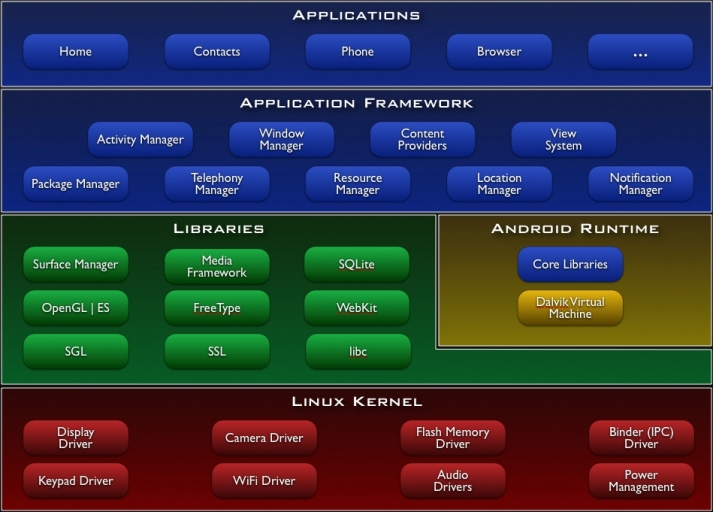
\includegraphics[width=0.7\columnwidth]{figs/system-architecture}
\caption{An overview of the Android system architecture, from \citep{androidarchitectureoverview}}
\label{fig:androidoverview}
\end{center}
\end{figure}


\section{Android Architecture Overview}
Android is an open-source project, built on Linux. Designed to be a lightweight, modular, extendable, and versatile operating system, Android removed almost all of the typical GNU/Linux stack, and wrote an entire framework from scratch. Built in Java, Android runs the Dalivk VM, a lightweight Java-compatible VM (see Figure \ref{fig:androidoverview}). 

The three major application components of Android are Activities, Services, and Content Providers. They are joined together through the Intent system. Activities are user-facing tasks, and follow the iOS definition of an ``app''. Only one may run at a time, and they have strict lifecycles. Services run in the background and follow a less strict lifecycle. Their main purpose is to perform long-running tasks that do not require user input. Lastly, Content Providers ``manage access to a structured set of data. They encapsulate the data, and provide mechanisms for defining data security. Content providers are the standard interface that connects data in one process with code running in another process''\citep{androidcontentproviders}.

Android was built from the ground-up to be composed of strongly isolated modules with little dependencies. No traditional SysV IPC is allowed; instead Android provides its own inter-app communication built off of its Intent system. Intents on Android, as described in the documentation, are ``an abstract description of an operation to be performed... An Intent provides a facility for performing late runtime binding between the code in different applications. Its most significant use is in the launching of activities, where it can be thought of as the glue between activities. It is basically a passive data structure holding an abstract description of an action to be performed''\citep{androidintents}. Intents allow apps to describe the operation they would like to perform, without explicitly identifying a recipient. For example, when the intent \textit{ACTION\_VIEW} is sent with data ``http://google.com'', Android searches through all installed apps that designate that they respond to that intent and will pick one to deliver it to; in this case, the \textit{Browser} would respond.

\section{Android Permissions}
The highly modular and decentralized aspect of Android makes it extremely easy to tap into virtually all Personally Identifiable Information on the device. To protect this, and many other aspects of the system, Android utilizes the Permission security model. The permission security model is a static list of capabilities an app possesses: when presented with this list before installation (see Figure \ref{fig:gpstorepermissions}), a user will either grant the app access to the features or simply not install the app. When an app requests a permission, the Android system treats it as if the user granted the app that capability. After installation, this list will never change unless the app package itself changes and the user reviews the new permissions.

\begin{figure}[h]
\begin{center}
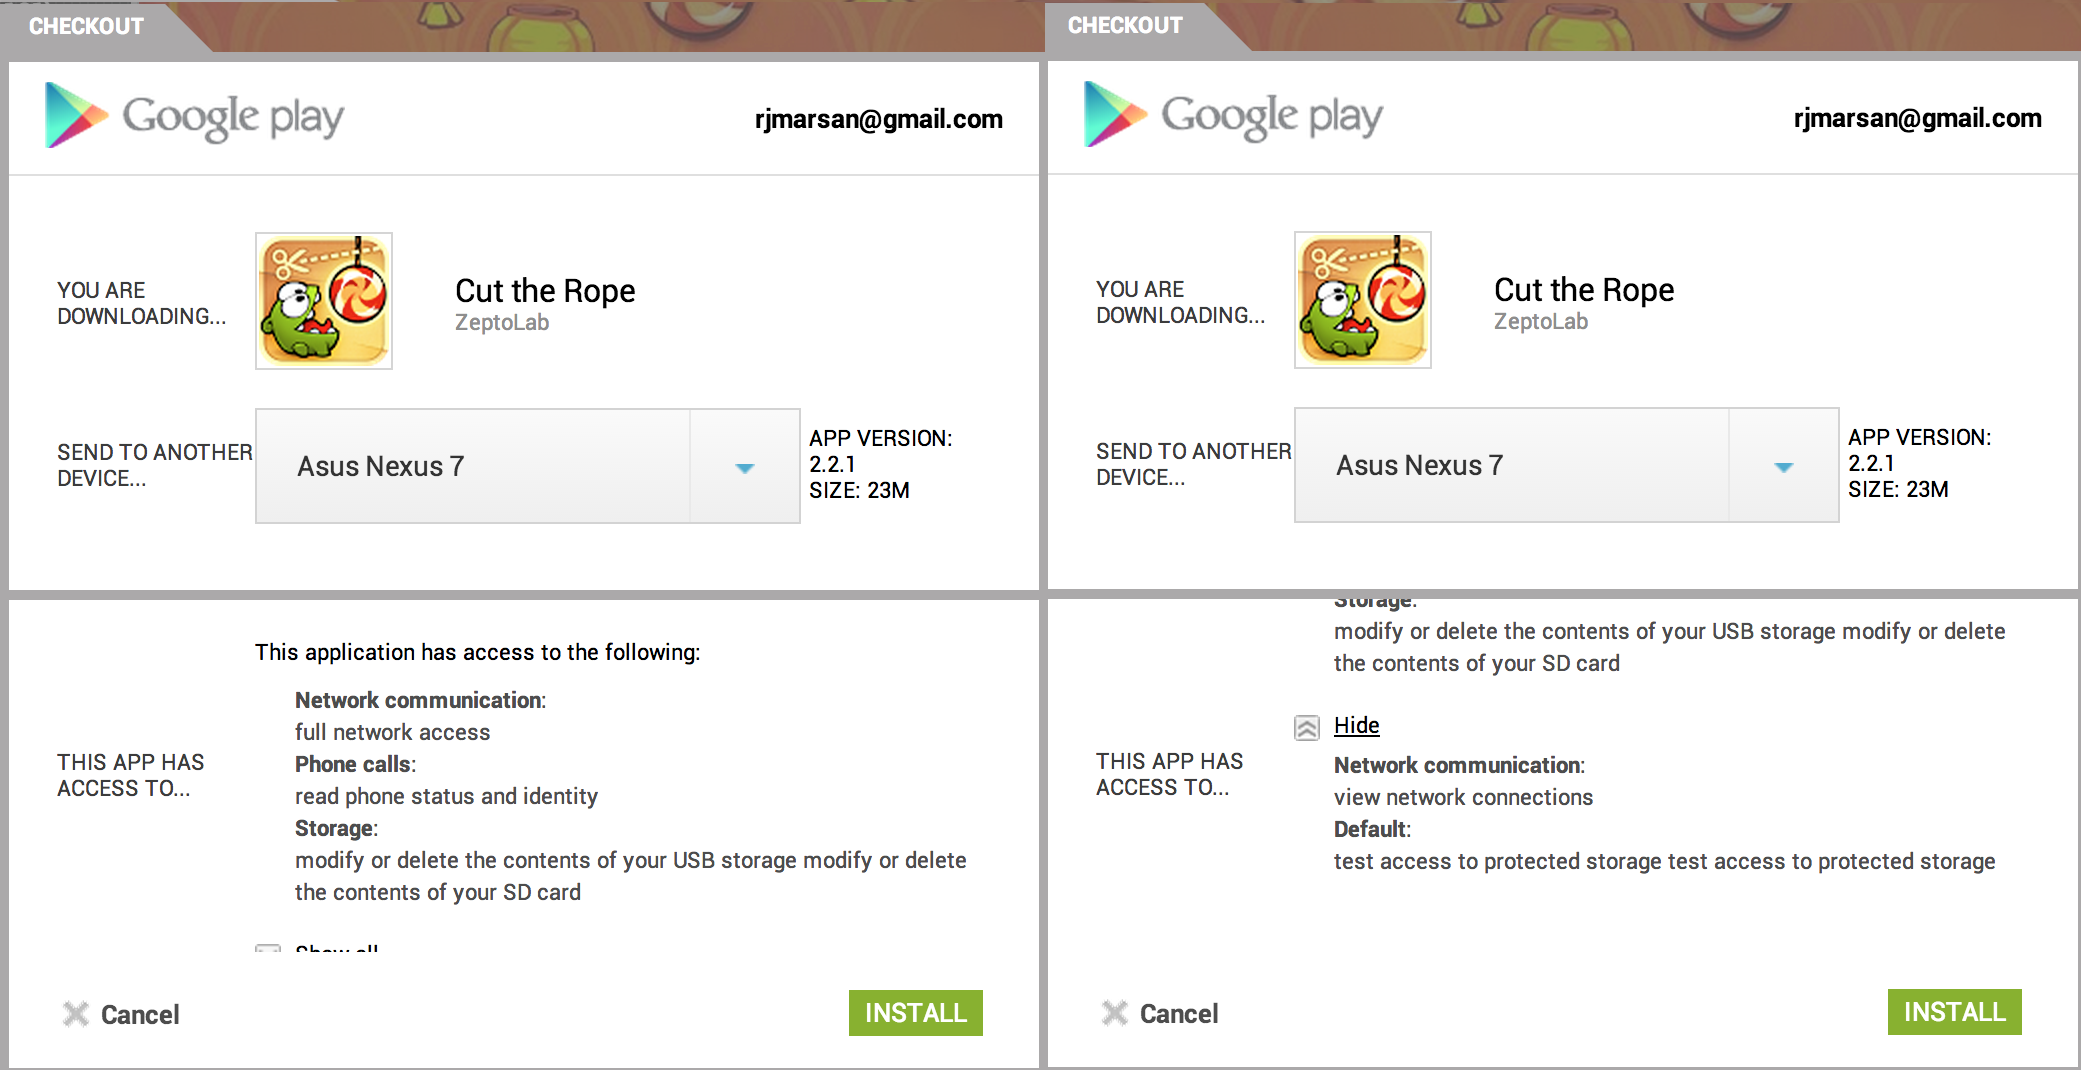
\includegraphics[width=1.0\columnwidth]{figs/GPStoreInstallScreen}
\caption{A sample Google Play Store install screen showing the permissions. The user must scroll to see all of them, and click ``Show All'' to see the hidden ones.}
\label{fig:gpstorepermissions}
\end{center}
\end{figure}

Android permissions themselves are much more granular than a typical UNIX permission system. They cover a wide variety of operations, including controlling the sleep state, accessing hardware, accessing PII, and many system operations. Some of the most requested permissions can be seen in Table \ref{tab:perms}; the rest can be seen in Appendix Table \ref{tab:allperms}.

%\begin{smitemize}
%\item \textit{android.permission.INTERNET}: Grants the app access to network sockets. Without this, an app alone could not access the internet over WiFi, 3G, or other interfaces. No restrictions are placed on the protocol, ports, or domains accessed.
%\item \textit{android.permission.WAKE\_LOCK}: Prevents the device from sleeping. When a Wake Lock is acquired, the Android system will not shut off. Depending the Wake Lock, the screen may continue to stay on, or it may turn off, but the CPU and other hardware remains in operation.
%\item \textit{android.permission.READ\_PHONE\_STATE}: Grants the app access to the phone hardware, which includes IMEI, GSM information, as well as the phone number of the current call. Since the IMEI is frequently used as a UDID, this is a popular permission.
%\item \textit{android.permission.CAMERA}: Allows apps access to the camera hardware, if present. The Android system still requires an app hold a valid drawing surface before data is sent to the app, making it difficult to perform in the background.
%\item \textit{android.permission.READ\_CONTACTS/READ\_SMS/READ\_CALENDAR}: offers read-only access to personal information. <say more?>
%\item \textit{android.permission.WRITE\_CONTACTS/WRITE\_SMS/WRITE\_CALENDAR}: offers write-only access to personal information. <say more?>
%\end{smitemize}





\begin{table*}[t]
\begin{small}
\begin{tabular}{p{3cm}|p{12.5cm}}
Permission  & Description \\
\hline

\textit{INTERNET} & Network communication. full Internet access. Allows the app to create network sockets.  \\
\textit{WRITE\_EXTERNAL\_\-STORAGE} & Storage. modify/delete USB storage contents modify/delete SD card contents. Allows the app to write to the USB storage.  Allows the app to write to the SD card.  \\
\textit{READ\_PHONE\_STATE} & Phone calls. read phone state and identity. Allows the app to access the phone features of the device.  An app with this permission can determine the phone number and serial number of this phone, whether a call is active, the number that call is connected to and the like.  \\
\textit{ACCESS\_FINE\_\-LOCATION} & Your location. fine (GPS) location. Access fine location sources such as the Global Positioning System on the tablet, where available.  Malicious apps may use this to determine where you are, and may consume additional battery power.  \\
\textit{ACCESS\_COARSE\_\-LOCATION} & Your location. coarse (network-based) location. Access coarse location sources such as the cellular network database to determine an approximate tablet location, where available.  Malicious apps may use this to determine approximately where you are. \\
\textit{WAKE\_LOCK} & System tools. prevent tablet from sleeping prevent phone from sleeping. \\
\textit{READ\_CONTACTS} & Your personal information. read contact data. Allows the app to read all of the contact (address) data stored on your tablet.  Malicious apps may use this to send your data to other people. \\
\textit{CALL\_PHONE} & Services that cost you money. directly call phone numbers. Allows the app to call phone numbers without your intervention.  Malicious apps may cause unexpected calls on your phone bill.  Note that this doesn't allow the app to call emergency numbers.  \\
\textit{CAMERA} & Hardware controls. take pictures and videos. Allows the app to take pictures and videos with the camera.  This allows the app at any time to collect images the camera is seeing.  \\
\textit{WRITE\_CONTACTS} & Your personal information. write contact data. Allows the app to modify the contact (address) data stored on your tablet.  Malicious apps may use this to erase or modify your contact data.  \\
\textit{GET\_TASKS} & System tools. retrieve running apps. Allows the app to retrieve information about currently and recently running tasks.  Malicious apps may discover private information about other apps.  \\
%\textit{WRITE\_SETTINGS} & System tools. modify global system settings. Allows the app to modify the system's settings data.  Malicious apps may corrupt your system's configuration.  \\
\textit{RECORD\_AUDIO} & Hardware controls. record audio. Allows the app to access the audio record path.  \\
\textit{SEND\_SMS} & Services that cost you money. send SMS messages. Allows the app to send SMS messages.  Malicious apps may cost you money by sending messages without your confirmation.  \\
\textit{READ\_HISTORY\_\-BOOKMARKS} & Your personal information. read Browser's history and bookmarks. Allows the app to read all the URLs that the Browser has visited, and all of the Browser's bookmarks.  \\
\textit{READ\_CALENDAR} & Your personal information. read calendar events plus confidential information. Allows the app to read all calendar events stored on your tablet, including those of friends or coworkers.  Malicious apps may extract personal information from these calendars without the owners' knowledge. \\
\textit{WRITE\_HISTORY\_\-BOOKMARKS} & Your personal information. write Browser's history and bookmarks. Allows the app to modify the Browser's history or bookmarks stored on your tablet.  Malicious apps may use this to erase or modify your Browser's data \\
\textit{RECEIVE\_SMS} & Your messages. receive SMS. Allows the app to receive and process SMS messages.  Malicious apps may monitor your messages or delete them without showing them to you.  \\
\textit{WRITE\_CALENDAR} & Your personal information. add or modify calendar events and send email to guests without owners' knowledge. Allows the app to send event invitations as the calendar owner and add, remove, change events that you can modify on your device, including those of friends or co-workers.  Malicious apps may send spam emails that appear to come from calendar owners, modify events without the owners' knowledge, or add fake events.  \\
%\textit{CHANGE\_WIFI\_STATE} & System tools. change Wi-Fi state. Allows the app to connect to and disconnect from Wi-Fi access points, and to make changes to configured Wi-Fi networks.  \\
%\textit{ACCESS\_MOCK\_LOCATION} & Your location. mock location sources for testing. Allows the app to create mock location sources for testing.  Malicious apps may use this to override the location and/or status returned by real location sources such as GPS or network providers.  \\
%\textit{PROCESS\_OUTGOING\_CALLS} & Phone calls. intercept outgoing calls. Allows the app to process outgoing calls and change the number to be dialed.  Malicious apps may monitor, redirect, or prevent outgoing calls.  \\
%\textit{MODIFY\_AUDIO\_SETTINGS} & Hardware controls. change your audio settings. Allows the app to modify global audio settings such as volume and routing.  \\
\textit{MOUNT\_UNMOUNT\_\-FILESYSTEMS} & System tools. mount and unmount filesystems. Allows the app to mount and unmount filesystems for removable storage.  \\
\textit{READ\_SMS} & Your messages. read SMS or MMS. Allows the app to read SMS messages stored on your tablet or SIM card.  Malicious apps may read your confidential messages. \\
\textit{READ\_LOGS} & Your personal information. read sensitive log data. Allows the app to read from the system's various log files.  This allows it to discover general information about what you are doing with the tablet, potentially including personal or private information.  \\
\textit{DISABLE\_KEYGUARD} & System tools. disable keylock. Allows the app to disable the keylock and any associated password security.  A legitimate example of this is the phone disabling the keylock when receiving an incoming phone call, then re-enabling the keylock when the call is finished.  \\
%\textit{BLUETOOTH} & Network communication. create Bluetooth connections. Allows the app to view the configuration of the local Bluetooth tablet, and to make and accept connections with paired devices. \\
%\textit{WRITE\_SMS} & Your messages. edit SMS or MMS. Allows the app to write to SMS messages stored on your tablet or SIM card.  Malicious apps may delete your messages. \\
%\textit{CHANGE\_CONFIGURATION} & System tools. change your UI settings. Allows the app to change the current configuration, such as the locale or overall font size.  \\

\end{tabular}
\end{small}
%\vspace{-0.2in}
\caption{Frequently Requested Android permissions, and the GPStore's description of them}
\label{tab:perms}
%\vspace{-0.1in}
\end{table*}





In cases like \textit{WAKE\_LOCK} and \textit{CAMERA}, the permission seems fairly singular: access to exactly one feature. However, for other permissions, such as \textit{INTERNET} and \textit{READ\_PHONE\_STATE}, many more granularities could be established. For example, \textit{INTERNET} gives unconditional access to all domains, unlike web pages in modern web browsers. In addition, while permissions are intended to be non-overlapping, there still are ways --- varying from minor to major --- to acquire information guarded by one permission from another. For example, \textit{READ\_PHONE\_STATE} can access to the current phone call, and is able to establish call logs, an operation normally protected by \textit{READ\_CONTACTS}. There are some permissions, however, that are explicitly supersets of another other, such as \textit{ACCESS\_COURSE\_LOCATION} --- providing network-tower location --- and its superset, \textit{ACCESS\_FINE\_LOCATION} --- providing GPS location. 

Permissions do not tend to change through Android's release history. As new hardware is made accessible through Android's SDK, new permissions are added for them, but there are very few times when permissions drastically change meaning or scope. Through Android's 6 year history, only 3 new permissions has been added to restrict previously unrestricted operations\footnote{In Android 4.1, the storage device requires a permission to read, and the call logs require a separate permission to read and write --- previously they shared a permission with contacts\citep{android41new}.}.

\section{Permission Enforcement}
Permission enforcement on Android is generally performed in two main ways: UNIX permissions and explicit runtime checking. Most hardware is accessible using C or other low-level calls, so permissions are more effectively enforced via UNIX Group Permissions. Upon app installation, Android assigns each app a unique UID and assigns different group permissions to that user. For example, socket access is granted to a UNIX group, and all apps that request \textit{INTERNET} are added to that group. This is simple, effective, and has very little performance overhead. Unfortunately, it makes it difficult to enforce when and how these resources are accessed. 

System operations --- like wake locks, changing system settings, turning on and off components, etc. --- are checked on every API call, through a centralized PackageManager class. The PackageManager first checks if the app has requested that permission. If it has, it then proceeds to check if the permission is protected by the system. Some permissions are only available to trusted code via either a shared key or being located in a system folder. Many system operations fall into this category, including \textit{WIPE\_DEVICE} and \textit{BRICK}. Typically, these operations are extremely dangerous and have the potential to destroy a device or perform elaborate phishing operations. Even if an app requests the permission, the PackageManager still has the right to reject the operation. This allows trusted developers access to system-level operations post-deployment on a device, while still protecting the operations from untrusted developers.

The final aspect of permissions deals with protecting PII. Android implements the bulk of PII sources through Content Providers, which manage a dataset and provide access to remote services. It is therefore imperative for each individual data source to check the permissions of the incoming app, every time it is requested. This, however, provides opportunities to extend its behavior.

\subsection{Permission Rejection}
\label{sec:permissionrejection}
When a permission is checked in Android, one of two outcomes is possible: (1) The check passes, and the operation continues as intended, or (2) the check fails and an exception is thrown. By design, the code path instantly jumps to an error state, halting the action. No logging of this action takes place, nor are partial passes allowed.

\section{Third Party Permissions}
\begin{sloppypar}
Android was built to distribute PII in a modular fashion, and it extended these features to other third party apps. Any developer may write Content Providers and, likewise, may create Permissions to protect them. Other apps must request that permission before accessing the data. For example: Alice writes a messaging app, \textit{MyMessenger}. She wants to expose the PII to other apps; so she makes a Content Provider around it. To protect the user's information, she defines her own permissions: \textit{mypackage.MyMessenger.READ\_MESSAGES} and \textit{mypackage.MyMessenger.WRITE\_MESSAGES}. Bob writes an app that uses \textit{MyMessenger}'s data to build a picture. His app requests the permission \textit{mypackage.MyMessenger.READ\_MESSAGES}. When his app contacts Alice's Content Provider, her app checks this custom permission before proceeding with the query. However, if Bob does not request \textit{mypackage.MyMessenger.WRITE\_MESSAGES} and attempts to perform a write action, Alice's Content Provider will reject the operation.
\end{sloppypar}
%These rejections are not logged or notified. expand on this.


If two apps request the same permissions, as long as neither have access to system permissions, it can be assumed that they have the same capabilities. Additionally, these capabilities are permanent, as permissions for a given package can not be added nor removed. This Permission Fingerprint, or set of capabilities, uniquely defines what an app has access to. All apps that request the same set of permissions have access to the exact same set of actions, and only through those permissions do they have those actions (with a few exceptions). Android permissions are static, however, and therefore a Permission Fingerprint doesn't guarantee a specific pattern of behavior. In fact, since not all permissions are guaranteed to be granted, a Permission Fingerprint simply establishes the absolute maximum capabilities of an app --- even if the system rejects some of them.
